\chapter{Lec 18 - Clustering}

\section{Clustering}
Clustering is the process of grouping a set of objects into groups of similar objects. It is the most common form of \textbf{unsupervised learning}, where we don't have a classification for the examples.\newline\newline
Given:
\begin{itemize}
    \item A set of instances $X = \{x_{1},....,x_{n}\}, x_{i} \in X$
    \item A measure of similarity
    \item A desired number of clusters $K$(optional)
\end{itemize}
Compute an assignment function $\gamma : X \rightarrow \{1,....,K\}$ such that no clusters are empty. $\gamma$ is a function that maps each instance in $X$ to one \footnote{there are also techniques that give a probability distribution for each instance over different clusters} of the clusters. Note that we use the term \textit{instances} rather than \textit{examples} because an example is usually a pair $(instance, label)$. Since in clustering we don't have labels, $X$ is a set of instances.\newline\newline
The clustering problem is an ill-posed problem. This is because the notion of group is vague and arbitrary (e.g. fruits can be clustered by shape or color and in both cases clustering would make perfect sense). Therefore, a crucial step to get good results from clustering is data representation. We need to represent data in such a way that similar objects have similar representations. When we choose a representation we are implicitly choosing a measure of similarity and vice versa (inductive bias). Another important choice to make in clustering is how many clusters we want. This parameter can be fixed in advance or can be completely data driven. In general, we want to avoid \textit{trivial} clusters (too big or too small).\newline\newline
Often, the goal of a clustering algorithm is to optimize an \textbf{objective function}. In theory, we could generate all possible clusterings, evaluate them and choose the one that optimizes the objective function. This method is not practical at all because there are too many possible clusterings ($\frac{K^{n}}{K!}$ where $n$ is the number of instances). So, clustering is a search (optimization) problem.\newline\newline
Most of clustering algorithms (e.g. k-means) start with an initial assignment and then refine it. The problem of having local minima in the objective function implies that different starting points can lead to very different (and not optimal) final partitions.

\section{Clustering evaluation}
How can we evaluate a clustering? There are two approaches:
\begin{itemize}
    \item \textbf{Internal criteria} which depends on the notion of similarity and/or on the chosen representation. We evaluate the intra-class similarity (the similarity between instances of the same cluster should be high) and the inter-class similarity (it should be low).
    \item \textbf{External criteria} that, given an \textbf{external} \textit{ground truth}, measures its proximity to the clustering we want to evaluate. 
\end{itemize}
\subsection{Internal methods for evaluation}
A clustering is a good clustering when it produces clusters in which:
\begin{itemize}
    \item the intra-class similarity (between examples in the same cluster) is high
    \item the inter-class similarity (between examples in different clusters) is low
\end{itemize}
Basically, we want to maximize the intra-class similarity and minimize the inter-class similarity. Note that this quality measure strongly depends on the chosen representation and on the similarity measure used. For example, an evaluation function $V$ could be defined as follows:
\[V(X,\gamma) = \sum_{k=1}^{K}\sum_{i:\gamma (x_{i})=k} ||x_{i} - c_{k}||^{2}\]
where $\gamma$ is the assignment and $c_{k}$ is the \textbf{centroid} of the k-th cluster (i.e. the mean of the instances assigned to the k-th cluster).

\subsection{External methods for evaluation}
The quality of a clustering is measured as the ability to recognize the hidden patterns and/or latent classes in the data. We have an external classification (\textit{ground truth}) for the data and we want to measure how much the clustering produced resembles this ground truth. Since evaluation methods used for classification are not directly usable, we need other techniques:
\begin{itemize}
    \item \textbf{Purity:} it is the ratio between the number of elements of the dominant \textbf{class} in a cluster (according to the ground truth classification) and the cardinality of the cluster. It's a good clustering when most of the clusters have all their instances of the same class in the ground truth. The total purity of the clustering will be the average of the purity of different clusters.
    \item \textbf{RandIndex:} it is similar to the notion of accuracy in classification. For each pair of examples, we evaluate the following statistics:
    \begin{itemize}
        \item A: number of pairs of the same class assigned to the same cluster (true positives)
        \item B: number of pairs of different class assigned to the same cluster (false positives)
        \item C: number of pairs of the same class assigned to different clusters (false negatives)
        \item D: number of pairs of different class assigned to different clusters (true negatives)
    \end{itemize}
    The RandIndex definition is given by:
    \[RI = \frac{A + D}{A + B + C + D}\]
    We can also consider measures corresponding to Precision and Recall, that is:
    \[P = \frac{A}{A+B} \quad \quad R = \frac{A}{A + C}\]
    There exists an extension of this method called \textbf{Adjusted RandIndex} ($ARI$):
    \[ARI = (RI - Expected\_RI) / (max(RI) - Expected\_RI)\]
    where $Expected\_RI$ is a random clustering. As you can see, this measure is always $< 1$ and it is $1$ only if $RI$ is the $max(RI)$. It can be $< 0$ if the clustering produced is \textit{worst} than a random clustering.
    \item \textbf{Other methods} such as entropy (or mutual information) among classes of the ground truth and the clusters produced.
\end{itemize}
\section{Clustering algorithms}
Let's start to introduce two different methods for clustering:
\begin{itemize}
    \item \textbf{Partitioning} (or flat) algorithms: they usually start with a random partition and iteratively refine it. On each step the objective function of the algorithm improves.
    \item \textbf{Hierarchical algorithms:} there are two different approaches:
    \begin{itemize}
        \item Bottom-up (or agglomerative) 
        \item Top-down (or divisive)
    \end{itemize}
\end{itemize}
\subsection{Partitioning algorithms}
Partitioning algorithms build a partition of $n$ instances in $K$ clusters (we need to define the number of clusters in advance). Given a set of instances and a number $K$, they find a $K$ clusters partition that optimizes a certain criterion. The overall optimal can be found by exhaustively enumerating all possible partitions and selecting the one that maximizes the criterion. This method is obviously inefficient and can't be implemented, so, usually, these kind of algorithms work on heuristics (k-means, k-medoids). There are also probabilistic or model-based methods: EM-type approaches (e.g. density measure $p(\textbf{x}) = \sum_{i=1}^{K}p(\textbf{x}|c_{i})p(c_{i})$)
\subsubsection{K-Means Algorithm}
In k-means the goal is to minimize, for each cluster, the average of the distances between the instances\footnote{we assume that the instances are represented as real-valued vectors} and the \textit{center} of the cluster (centroid). A centroid is computed as follows:
\[\mu(c) = \frac{1}{|c|}\sum_{x \in c}x\]
Instances are assigned to clusters according to the \textit{nearest} centroid.\newline\newline
\textbf{K-means algorithm:}
\begin{enumerate}
    \item Generate $K$ points (seeds) in the space. These points represent the initial centroids (e.g. $K$ randomly chosen instances);
    \item Assign each instance to the cluster whose centroid is the closest according to the considered similarity/distance measure;
    \item After assigning all the instances, recompute each cluster center as the mean of all the instances assigned to it;
    \item Repeat steps 2 and 3 until the centroids stabilize.
\end{enumerate}
It can be shown that, at each execution of steps 2 and 3, the value of the objective function is reduced:
\[V(X,\gamma) = \sum_{k=1}^{K}\sum_{i:\gamma (x_{i})=k} ||x_{i} - c_{k}||^{2}\]
\subsection{Hierarchical algorithms}
When the optimal number of clusters is not given, we can use hierarchical algorithms. The idea is to build a tree-based taxonomy from a set of instances that represents the cluster structure (dendrogram).\newline\newline
A first approach is to consider the recursive application of a partitioning clustering algorithm (divisive or top-down methods). These algorithms start from one single cluster that contains all the instances and partition it in multiple clusters.\newline\newline
A second (more popular) approach is through aggregation of clusters in a bottom-up mode. Initially, we have one cluster for each instance, and then we merge different clusters until we reach just one cluster.
\subsubsection{Agglomerative Hierarchical Clustering (HAC)}
Let's start with singleton clusters, one for each instance. Then, we gradually merge the closest pairs of clusters until we obtain a single cluster. The \textit{history} of merges forms a binary tree or hierarchy (dendrogram).
\begin{center}
    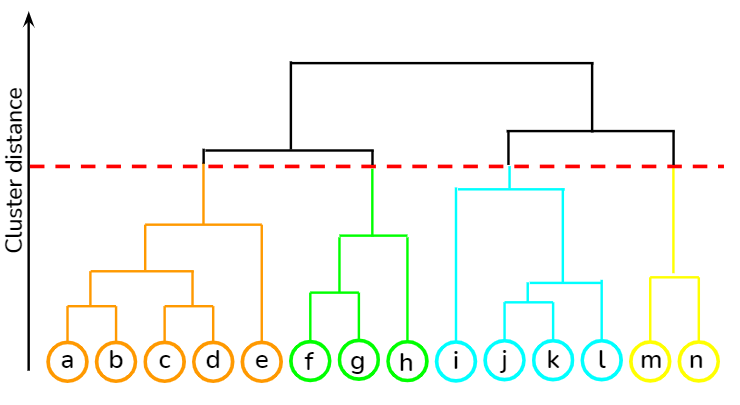
\includegraphics[scale=0.4]{images/HAC.png}
\end{center}
The $y$ axis of the dendrogram represents the similarity of the combination, that is, with which similarity the two clusters have been merged. The clustering is obtained by \textit{"cutting"} the dendrogram to the desired level. Each connected component under a certain threshold is a cluster.\newline\newline 
How can we measure the distance between two clusters? There are different methods:
\begin{itemize}
    \item \textbf{Single-link:} Similarity between the most similar instances in the clusters. It tends to aggregate all the closest instances and produce \textit{"elongated"} clusters (chaining effect).
    \item \textbf{Complete-link:} Similarity between the most distant instances in the clusters. It is sensitive to outliers.
    \item \textbf{Centroid:} Similarity between the centroids of the clusters. Note that the merge operation is assumed to be monotone, that is, if $s_{1},....,s_{k}$ are successive similarities obtained by the merge, then $s_{1} > s_{2} > ... > s_{k}$. With the centroid measure this is not always the case.
    \item \textbf{Average-link:} Mean similarity between pairs of instances of clusters. It computes the similarities between all the possible pairs of instances between the two clusters and averages these values.
\end{itemize}
\begin{center}
    \begin{tabular}{|c|c|c|c|}
     \hline
     \textbf{Name} & \textbf{Description} & \textbf{Complexity} & \textbf{Pros/Cons}\\
     \hline
     Single-link & Max sim. of any two points & $O(N^{2})$ & Chaining effect \\
     \hline
     Complete-link & Min sim. of any two points & $O(N^{2}logN)$ & Sensitive to outliers \\
     \hline
     Centroid & Similarity of centroids & $O(N^{2}logN)$ & Non monotonic \\
     \hline
     Group-average & Avg. sim. of any two points & $O(N^{2}logN)$ & OK\\
     \hline
\end{tabular}
\end{center}
